\documentclass[a4]{article}
\pagestyle{myheadings}

%%%%%%%%%%%%%%%%%%%
% Packages/Macros %
%%%%%%%%%%%%%%%%%%%
\usepackage{mathrsfs}


\usepackage{fancyhdr}
\pagestyle{fancy}
\lhead{}
\chead{}
\rhead{}
\lfoot{}
\cfoot{} 
\rfoot{\normalsize\thepage}
\renewcommand{\headrulewidth}{0pt}
\renewcommand{\footrulewidth}{0pt}
\newcommand{\RomanNumeralCaps}[1]
    {\MakeUppercase{\romannumeral #1}}

\usepackage{amssymb,latexsym}  % Standard packages
\usepackage[utf8]{inputenc}
\usepackage[russian]{babel}
\usepackage{MnSymbol}
\usepackage{mathrsfs}
\usepackage{amsmath,amsthm}
\usepackage{indentfirst}
\usepackage{graphicx}%,vmargin}
\usepackage{graphicx}
\graphicspath{{pictures/}} 
\usepackage{verbatim}
\usepackage{color}
\usepackage[nottoc,numbib]{tocbibind}
\usepackage{float}

\usepackage{listings}
\definecolor{codegreen}{rgb}{0,0.6,0}
\definecolor{codegray}{rgb}{0.5,0.5,0.5}
\definecolor{codepurple}{rgb}{0.58,0,0.82}
\definecolor{backcolour}{rgb}{0.95,0.95,0.92}
 
\lstdefinestyle{mystyle}{
    backgroundcolor=\color{backcolour},   
    commentstyle=\color{codegreen},
    keywordstyle=\color{magenta},
    numberstyle=\tiny\color{codegray},
    stringstyle=\color{codepurple},
    basicstyle=\footnotesize,
    breakatwhitespace=false,         
    breaklines=true,                 
    captionpos=b,                    
    keepspaces=true,                 
    numbers=left,                    
    numbersep=5pt,                  
    showspaces=false,                
    showstringspaces=false,
    showtabs=false,                  
    tabsize=2
}
 
\lstset{style=mystyle}

\usepackage{url}
\urldef\myurl\url{foo%.com}





\DeclareGraphicsExtensions{.pdf,.png,.jpg}% -- настройка картинок

\usepackage{epigraph} %%% to make inspirational quotes.
\usepackage[all]{xy} %for XyPic'a
\usepackage{color} 
\usepackage{amscd} %для коммутативных диграмм
%\usepackage[colorlinks,urlcolor=red]{hyperref}

%\renewcommand{\baselinestretch}{1.5}
%\sloppy
%\usepackage{listings}
%\lstset{numbers=left}
%\setmarginsrb{2cm}{1.5cm}{1cm}{1.5cm}{0pt}{0mm}{0pt}{13mm}


\newtheorem{Lemma}{Лемма}[section]
\newtheorem{Proposition}{Предложение}[section]
\newtheorem{Theorem}{Теорема}[section]
\newtheorem{Corollary}{Следствие}[section]
\newtheorem{Remark}{Замечание}[section]
\newtheorem{Definition}{Определение}[section]
\newtheorem{Designations}{Обозначение}[section]




%%%%%%%%%%%%%%%%%%%%%%% 
%Подготовка оглавления% 
%%%%%%%%%%%%%%%%%%%%%%% 
\usepackage[titles]{tocloft}
\renewcommand{\cftdotsep}{2} %частота точек
\renewcommand\cftsecleader{\cftdotfill{\cftdotsep}}
\renewcommand{\cfttoctitlefont}{\hspace{0.38\textwidth} \LARGE\bfseries} 
\renewcommand{\cftsecaftersnum}{.}
\renewcommand{\cftsubsecaftersnum}{.}
\renewcommand{\cftbeforetoctitleskip}{-1em} 
\renewcommand{\cftaftertoctitle}{\mbox{}\hfill \\ \mbox{}\hfill{\footnotesize Стр.}\vspace{-0.5em}} 
%\renewcommand{\cftchapfont}{\normalsize\bfseries \MakeUppercase{\chaptername} } 
%\renewcommand{\cftsecfont}{\hspace{1pt}} 
\renewcommand{\cftsubsecfont}{\hspace{1pt}} 
%\renewcommand{\cftbeforechapskip}{1em} 
\renewcommand{\cftparskip}{3mm} %определяет величину отступа в оглавлении
\setcounter{tocdepth}{5} 
\renewcommand{\listoffigures}{\begingroup %добавляем номер в список иллюстраций
\tocsection
\tocfile{\listfigurename}{lof}
\endgroup}
\renewcommand{\listoftables}{\begingroup %добавляем номер в список иллюстраций
\tocsection
\tocfile{\listtablename}{lot}
\endgroup}


   
   
%\renewcommand{\thelikesection}{(\roman{likesection})}
%%%%%%%%%%%
% Margins %
%%%%%%%%%%%
\addtolength{\textwidth}{0.7in}
\textheight=630pt
\addtolength{\evensidemargin}{-0.4in}
\addtolength{\oddsidemargin}{-0.4in}
\addtolength{\topmargin}{-0.4in}

%%%%%%%%%%%%%%%%%%%%%%%%%%%%%%%%%%%
%%%%%%Переопределение chapter%%%%%% 
%%%%%%%%%%%%%%%%%%%%%%%%%%%%%%%%%%%
\newcommand{\empline}{\mbox{}\newline} 
\newcommand{\likechapterheading}[1]{ 
\begin{center} 
\textbf{\MakeUppercase{#1}} 
\end{center} 
\empline} 

%%%%%%%Запиливание переопределённого chapter в оглавление%%%%%% 
\makeatletter 
\renewcommand{\@dotsep}{2} 
\newcommand{\l@likechapter}[2]{{\bfseries\@dottedtocline{0}{0pt}{0pt}{#1}{#2}}} 
\makeatother 
\newcommand{\likechapter}[1]{ 
\likechapterheading{#1} 
\addcontentsline{toc}{likechapter}{\MakeUppercase{#1}}} 




\usepackage{xcolor}
\usepackage{hyperref}
\definecolor{linkcolor}{HTML}{000000} % цвет ссылок
\definecolor{urlcolor}{HTML}{3643FF} % цвет гиперссылок
 
\hypersetup{pdfstartview=FitH,  linkcolor=linkcolor,urlcolor=urlcolor, colorlinks=true}

%%%%%%%%%%%%
% Document %
%%%%%%%%%%%%

%%%%%%%%%%%%%%%%%%%%%%%%%%%%%
%%%%%%главы -- section*%%%%%%
%%%%section -- subsection%%%%
%subsection -- subsubsection%
%%%%%%%%%%%%%%%%%%%%%%%%%%%%%
\def \newstr {\medskip \par \noindent} 



\begin{document}
\def\contentsname{\LARGE{Содержание}}
\thispagestyle{empty}
\begin{center} 
	
\vspace{2cm} 
{\Large \sc Санкт-Петербургский Политехнический}\\
\vspace{2mm}
{\Large \sc Университет} им. {\Large\sc Петра Великого}\\
\vspace{1cm}
{\large \sc Институт прикладной математики и механики\\ 
\vspace{0.5mm}
\textsc{}}\\ 
\vspace{0.5mm}
{\large\sc Кафедра прикладной математики}\\
\vspace{15mm}
%\rule[0.5ex]{\linewidth}{2pt}\vspace*{-\baselineskip}\vspace*{3.2pt} 
%\rule[0.5ex]{\linewidth}{1pt}\\[\baselineskip] 
{\huge \sc Лабораторная работа №$4$\\
	Эмпирические функции и ядерные оценки
	\vspace{6mm}
	
}
\vspace*{2mm}
%\rule[0.7ex]{\linewidth}{1pt}\vspace*{-\baselineskip}\vspace{3.2pt} 
%\rule[0.5ex]{\linewidth}{2pt}\\ 
\vspace{6cm} 
Студент группы $3630102/70301$ \hfill Камянский Д.В.\\
\vspace{1cm}
Преподаватель \hfill Баженов А. Н.\\
\vspace{20mm} 


\vfill {\large\textsc{Санкт-Петербург}}\\ 
2020 г.
\end{center}

%%%%%%%%%%%%%%%%%%%%%%%%%%%%%%%%%%%%%%%%%%%%%%%%%%%%%%%%%%%%%%%%%%%%%%%%%%%%%%%%%%%%%%%%%%%%%%
%\ \\[4cm]

%\rm
%%%%%%%%%%%%%%%%%%%%%%%%%%%%%%%%%%%%%%%%%%%%%%%%%%%%%%%%%%%%%%%%%%%%%%%%%%%%%%%%%%%%%%%%%%%%%%
\newpage
\pagestyle{plain}

%\begin{center}
%\begin{abstract} 

%\end{abstract}

%\end{center}

\newpage
\tableofcontents{}
\newpage
\listoffigures{}
\listoftables{}
\newpage

\section{Постановка задачи}

Сгенерировать выборки размером 20, 60 и 100 элементов.
Построить на них эмпирические функции распределения и ядерные
оценки плотности распределения на отрезке $[-4, 4]$ , для непрерывных
распределений и на отрезке $[6, 14]$ , для распределения Пуассона.


Распределения:
\begin{equation}\label{eqn:normal}
N(x,0,1) = \frac{1}{\sqrt{2\pi}}e^{-\frac{x^2}{2}}
\end{equation} 

\begin{equation}\label{eqn:cauchy}
C(x,0,1) = \frac{1}{\pi(1+x^2)}
\end{equation}

\begin{equation}\label{eqn:laplace}
L\left( x,0,\frac{1}{\sqrt{2}}\right) = \frac{1}{\sqrt{2}}e^{-\sqrt{2}\vert x\vert}
\end{equation}

\begin{equation}\label{eqn:poisson}
P(5,k) = \frac{5^k}{k!}e^{-5}
\end{equation}  

\begin{equation}\label{eqn:uniform}
M(x,-\sqrt{3}, \sqrt{3}) = 
\begin{cases}
\frac{1}{2\sqrt{3}} &\vert x\vert \leqslant \sqrt{3}\\
0 &\vert x\vert > \sqrt{3}
\end{cases}
\end{equation}


\section{Теория}

Статистическим рядом называется последовательность различных элементов выборки $z_{1}, z_{2}, ... , z_{k}$, расположенных в возрастающем порядке с указанием частот $n_{1}, n_{2}, ... , n_{k}$, с которыми эти элементы содержатся в выборке.

Эмпирическая функция распределения:
\begin{equation}
F^{*}(x) = \dfrac{1}{n}\sum\limits_{z_{i}<x}n_{i}
\end{equation}
Ядерная оценка плотности:
\begin{equation}
f_h(x) = \frac{1}{nh}\sum\limits_{i=1}^nK\left(\frac{x-x_i}{h}\right)\label{eqn:art}
\end{equation}
где $K$ является ядром, а $h>0$ является сглаживающим параметром, и называется шириной полосы.

В данной работе в качестве ядра была выбрана плотность вероятности стандартного нормального распределения:
\begin{equation}
K(x) = \frac{1}{\sqrt{2\pi}}e^{-\frac{x^2}{2}}
\end{equation}

Параметр сглаживания будем выбирать по правилу Сильвермана
\begin{equation}
h_{n} = 1.06*\sigma*n^{-1/5}
\end{equation}
где $ \sigma $ - выборочное стандартное отклонение.

\section{Реализация}
Для генерации выборки был использован $Python\;3.8.2$: модуль $stats$ библиотеки $scipy$ для генерации выборок различных распределений и библиотека $matplotlib$ для построения графиков

\newpage
\section{Результаты}
\subsection{Эмпирические функции распределения}
\begin{center}

\begin{figure}[H]
\caption{Ядерная функция плотности для нормального распределения n = $20$ }
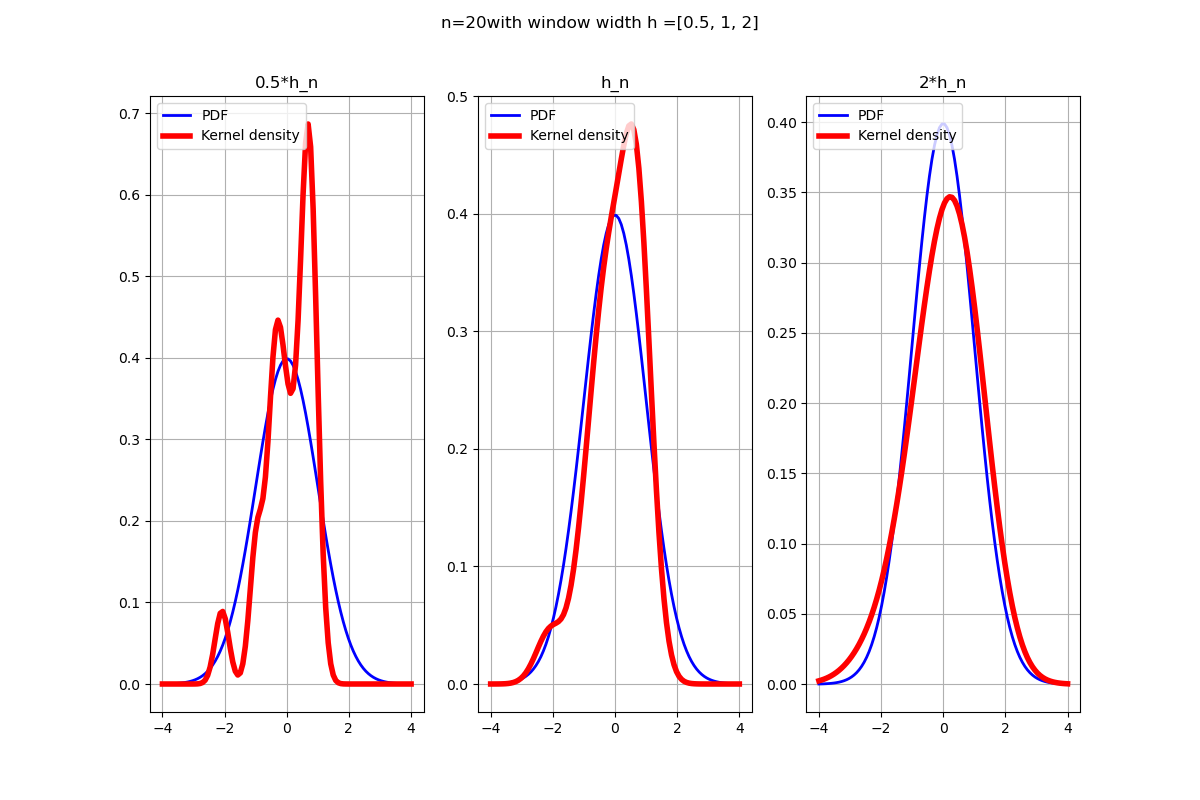
\includegraphics[width=\textwidth]{normal_pdf_20.png}
\end{figure}

\begin{figure}[H]
	\caption{Ядерная функция плотности для нормального распределения n = $60$ }
	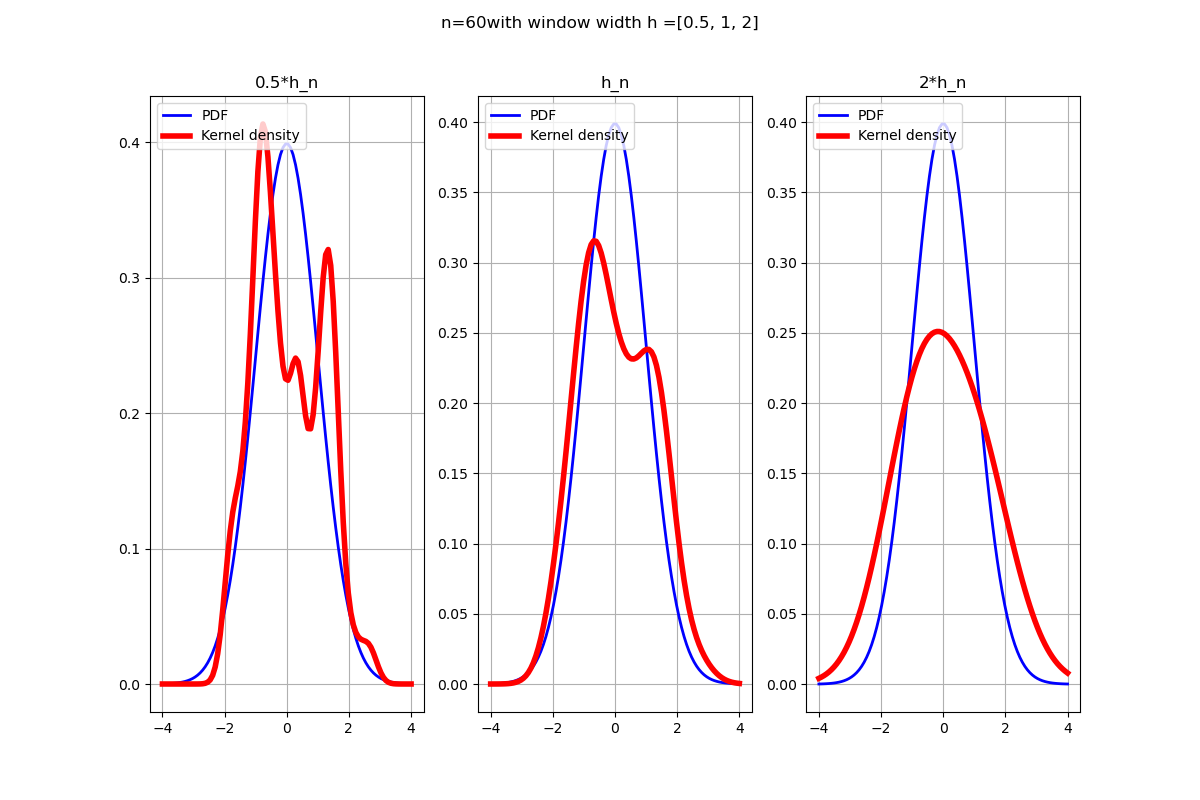
\includegraphics[width=\textwidth]{normal_pdf_60.png}
\end{figure}

\begin{figure}[H]
	\caption{Ядерная функция плотности для нормального распределения n = $100$ }
	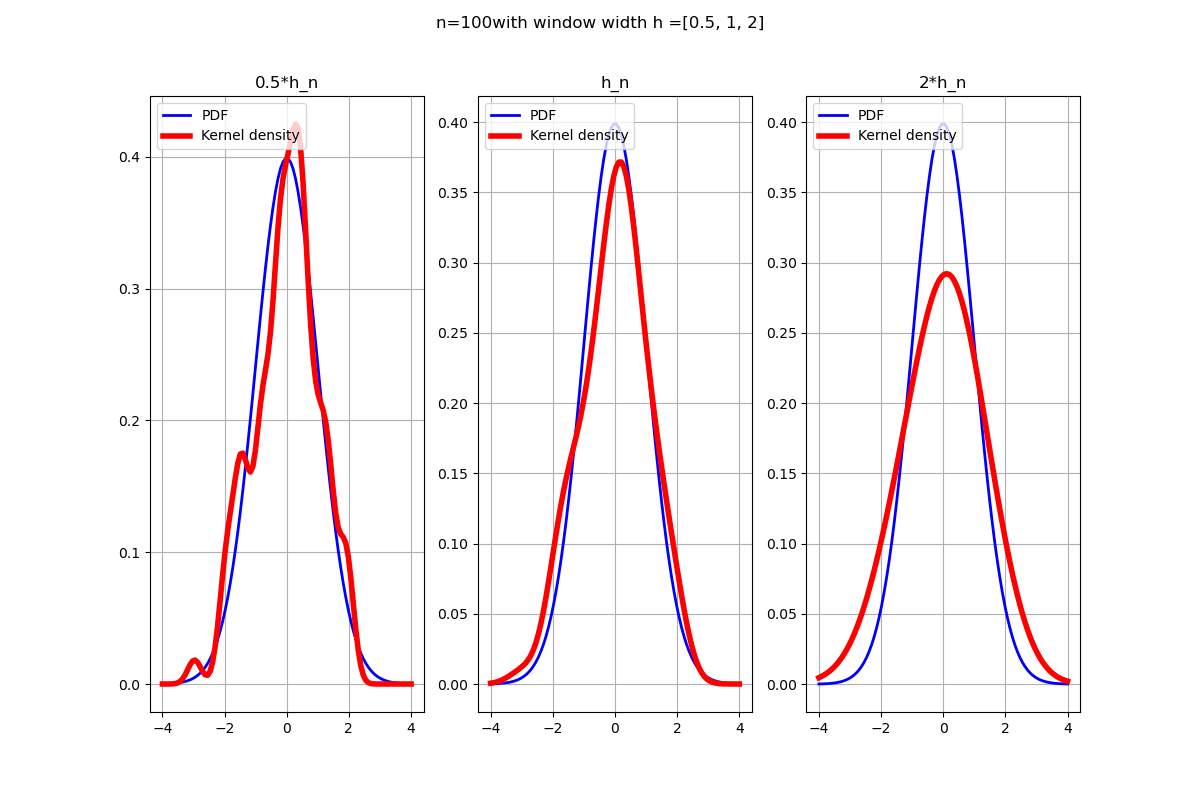
\includegraphics[width=\textwidth]{normal_pdf_100.png}
\end{figure}

\begin{figure}[H]
	\caption{Ядерная функция плотности для распределения Лапласа n = $20$ }
	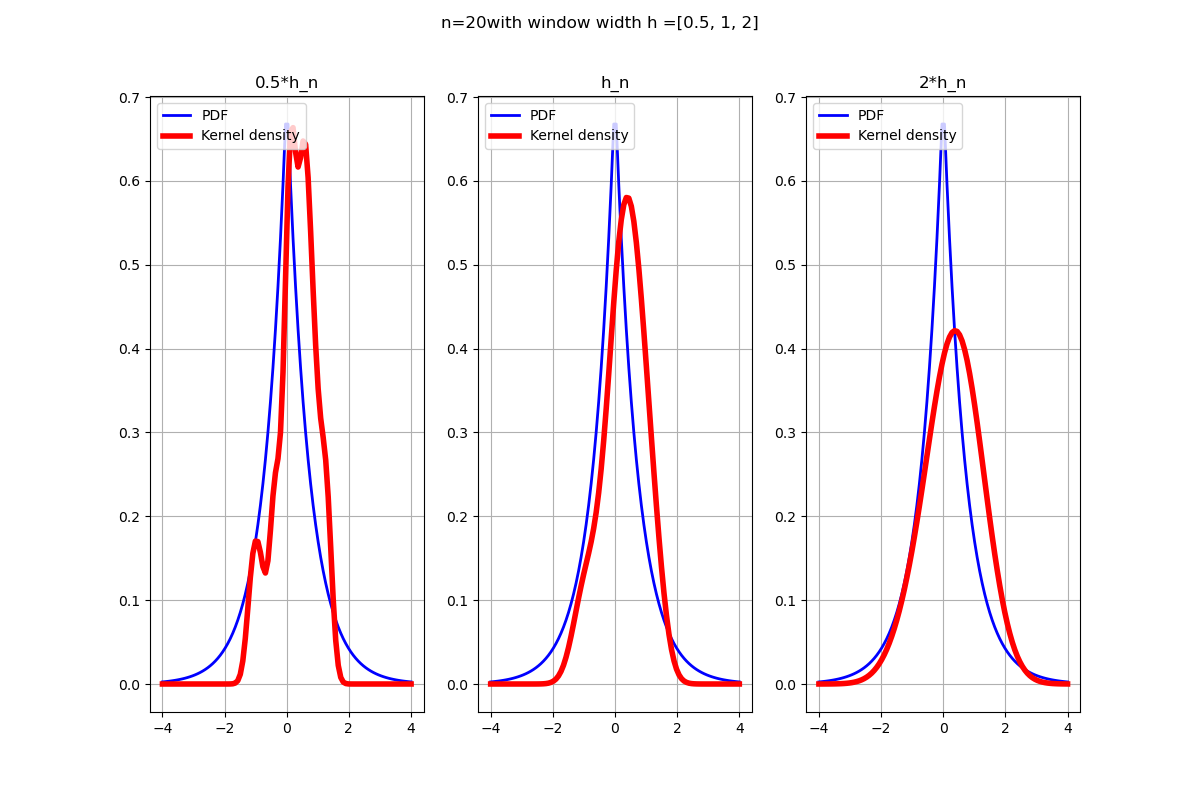
\includegraphics[width=\textwidth]{laplace_pdf_20.png} 
\end{figure}

\begin{figure}[H]
	\caption{Ядерная функция плотности для распределения Лапласа n = $60$ }
	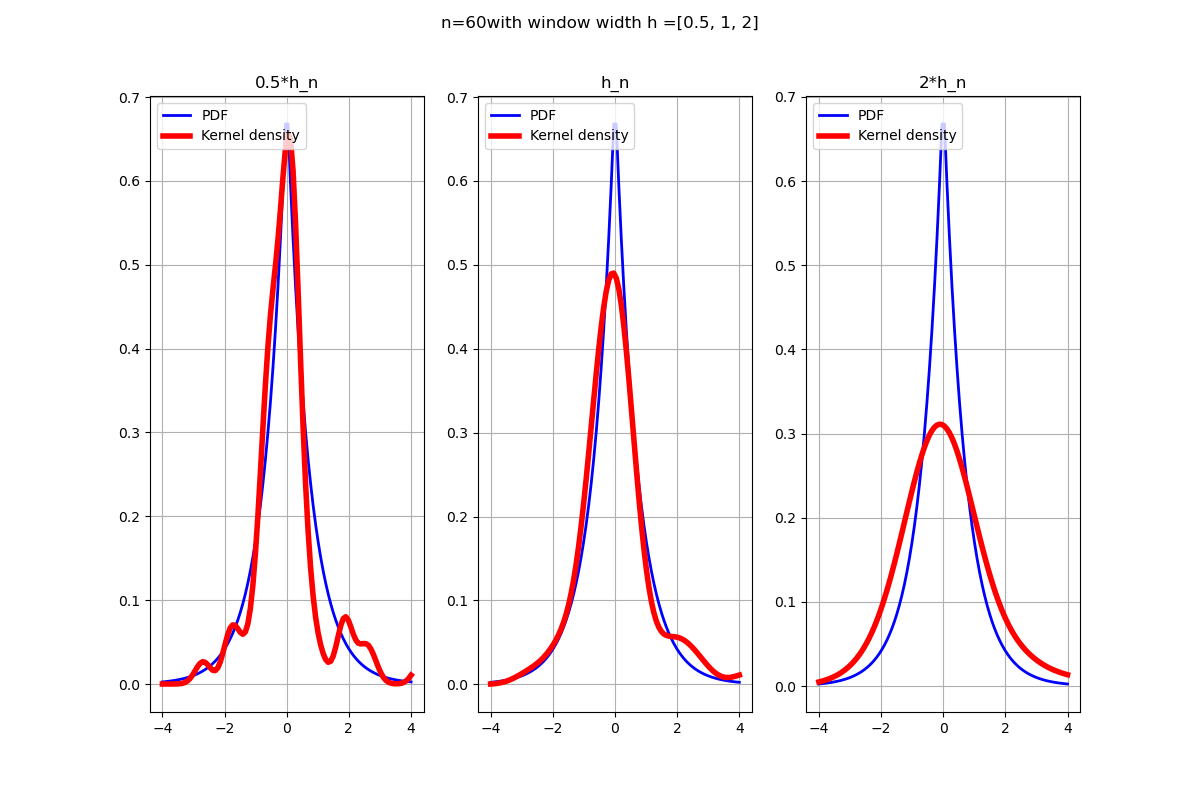
\includegraphics[width=\textwidth]{laplace_pdf_60.png} 
\end{figure}

\begin{figure}[H]
	\caption{Ядерная функция плотности для распределения Лапласа n = $100$ }
	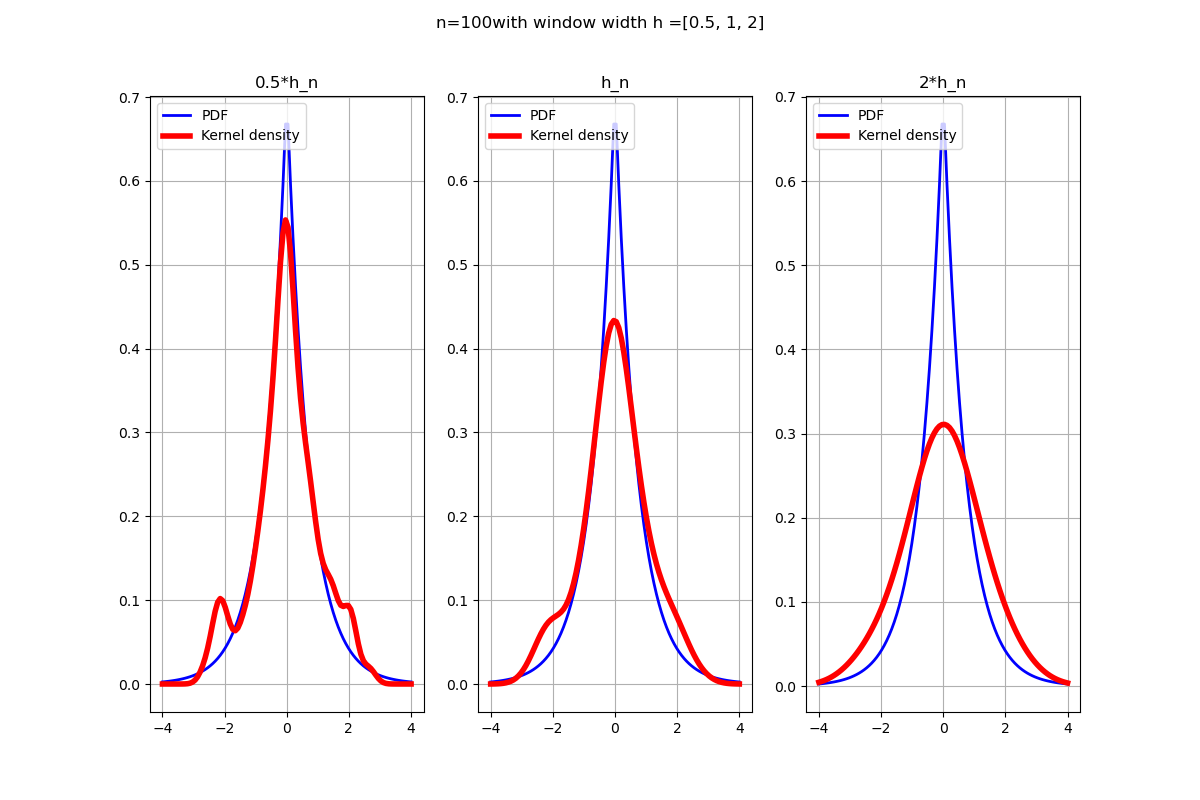
\includegraphics[width=\textwidth]{laplace_pdf_100.png} 
\end{figure}

\begin{figure}[H]
\caption{Ядерная функция плотности для распределения Коши n = $20$ }
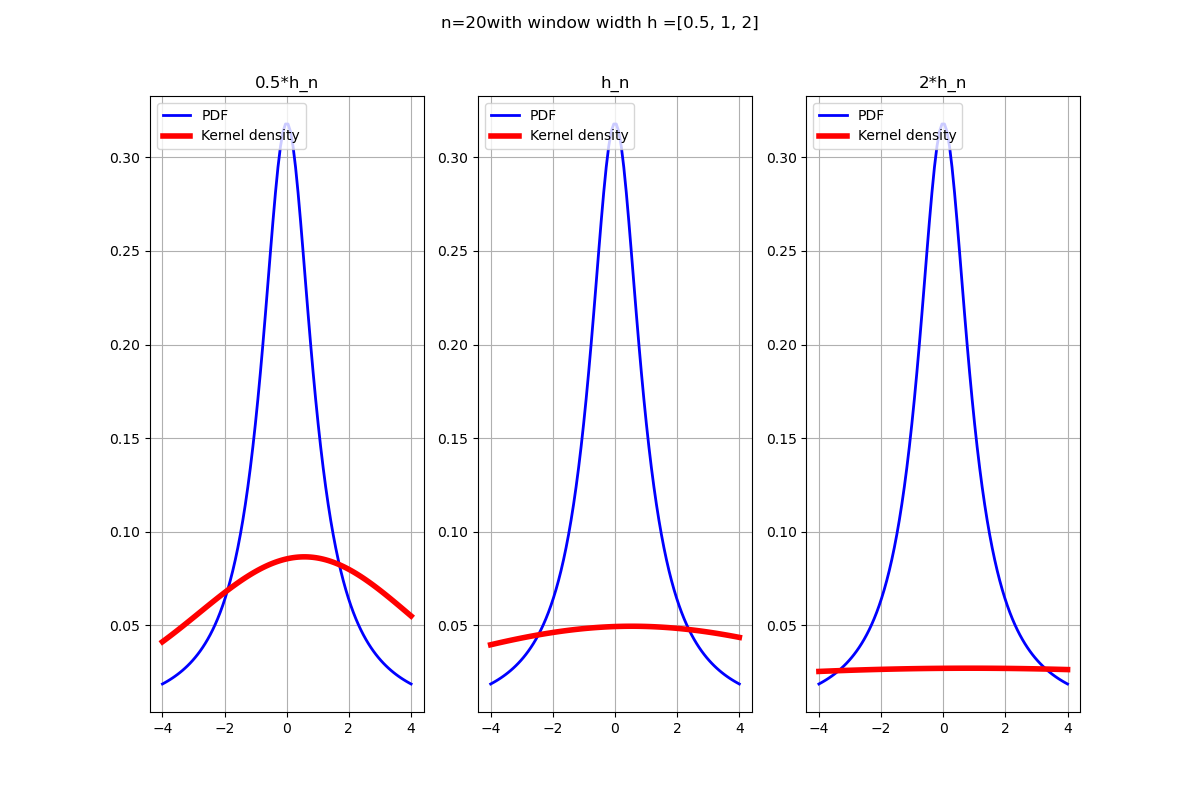
\includegraphics[width=\textwidth]{cauchy_pdf_20.png} 
\end{figure}

\begin{figure}[H]
	\caption{Ядерная функция плотности для распределения Коши n = $60$ }
	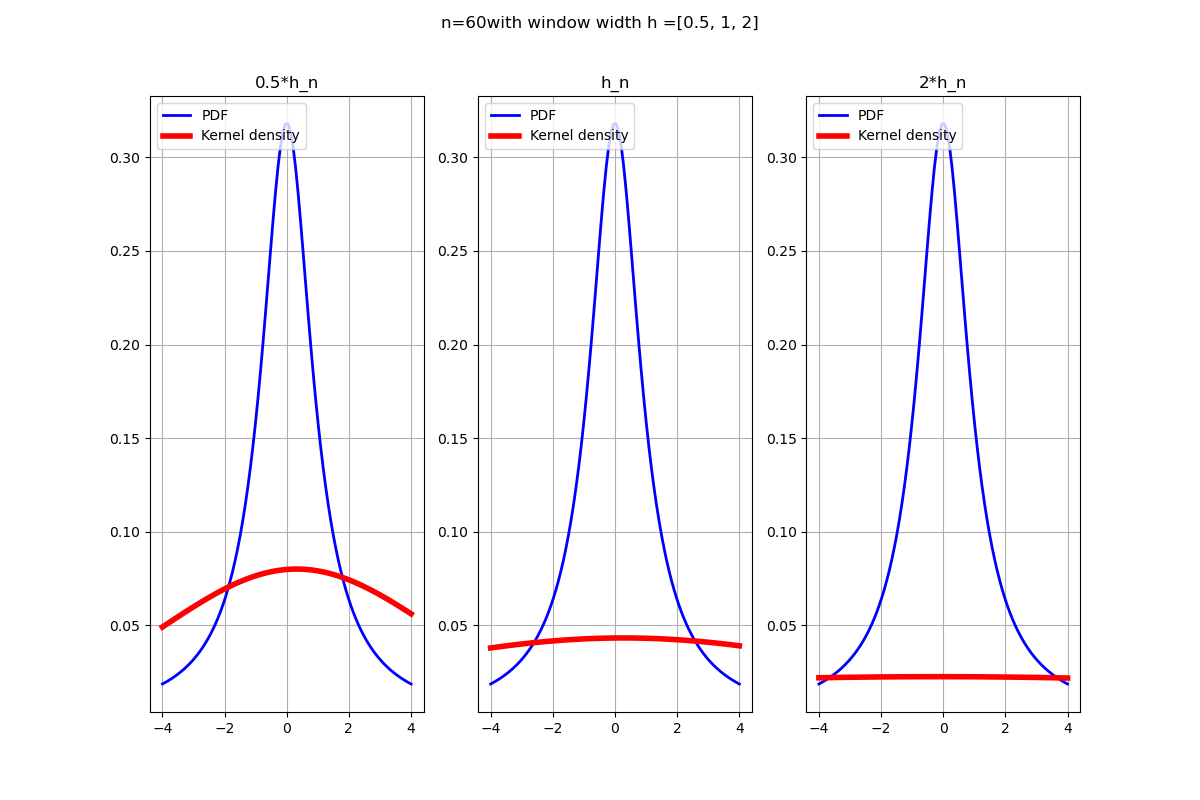
\includegraphics[width=\textwidth]{cauchy_pdf_60.png} 
\end{figure}

\begin{figure}[H]
	\caption{Ядерная функция плотности для распределения Коши n = $100$ }
	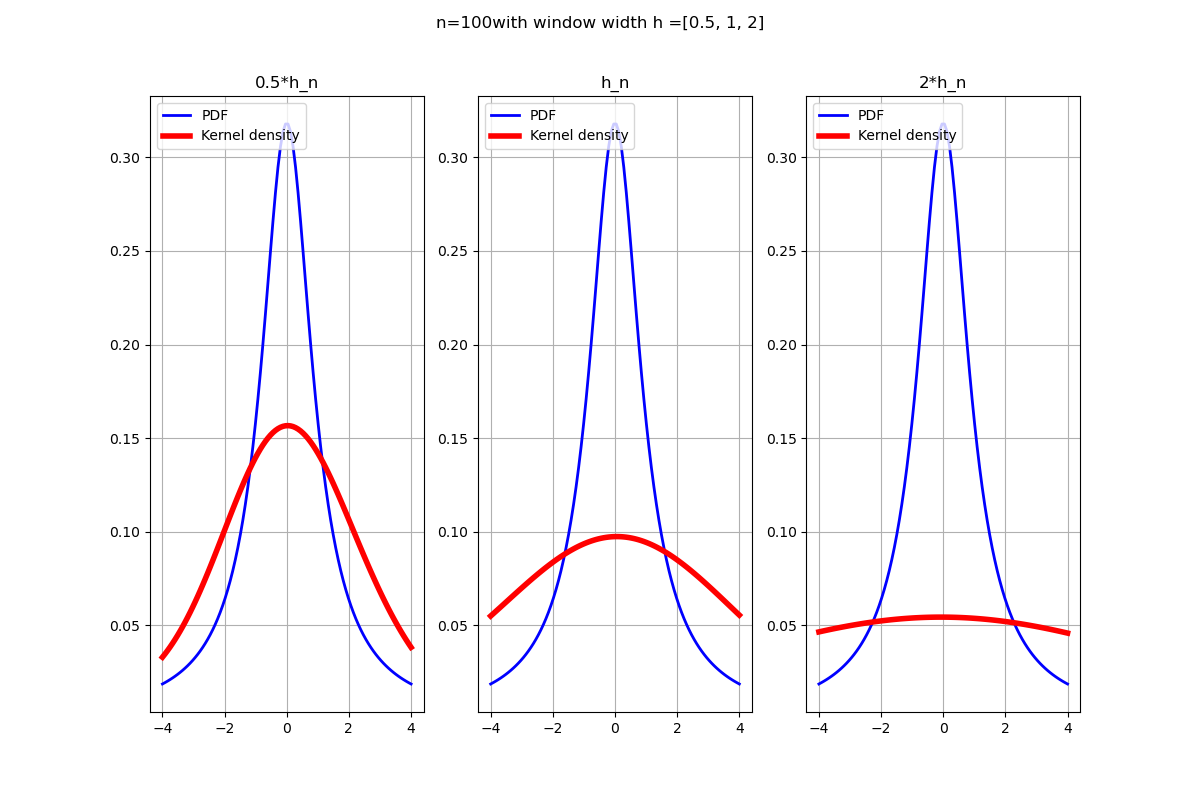
\includegraphics[width=\textwidth]{cauchy_pdf_100.png} 
\end{figure}

\begin{figure}[H]
\caption{Ядерная функция плотности для распределения Пуассона n = $20$}
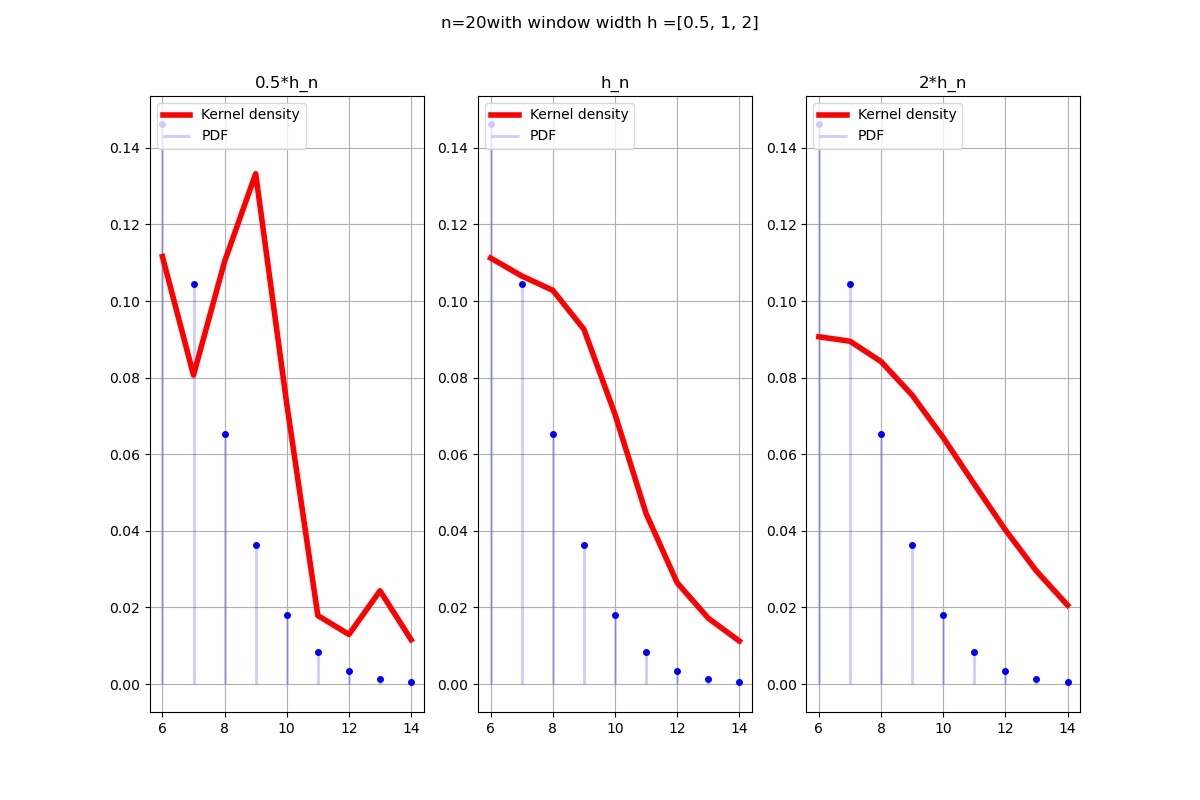
\includegraphics[width=\textwidth]{poisson_pdf_20.png} 
\end{figure}

\begin{figure}[H]
	\caption{Ядерная функция плотности для распределения Пуассона n = $60$}
	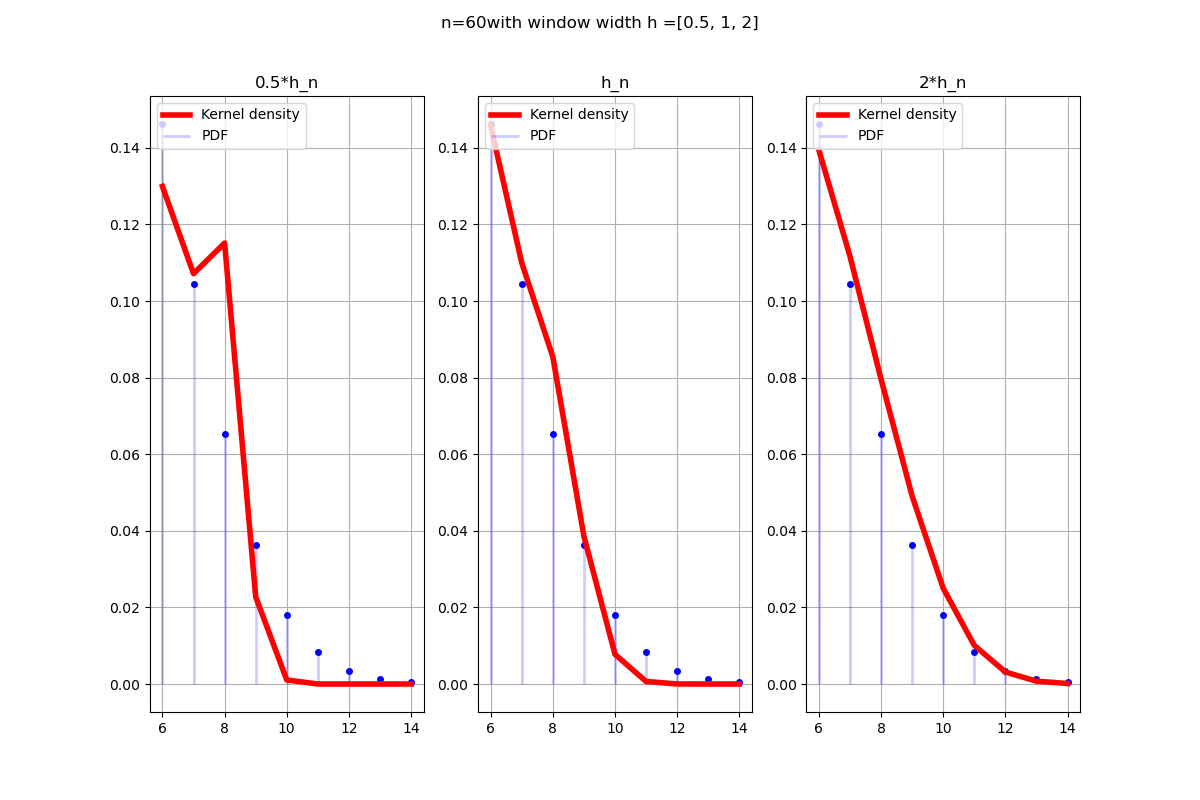
\includegraphics[width=\textwidth]{poisson_pdf_60.png} 
\end{figure}

\begin{figure}[H]
	\caption{Ядерная функция плотности для распределения Пуассона n = $100$}
	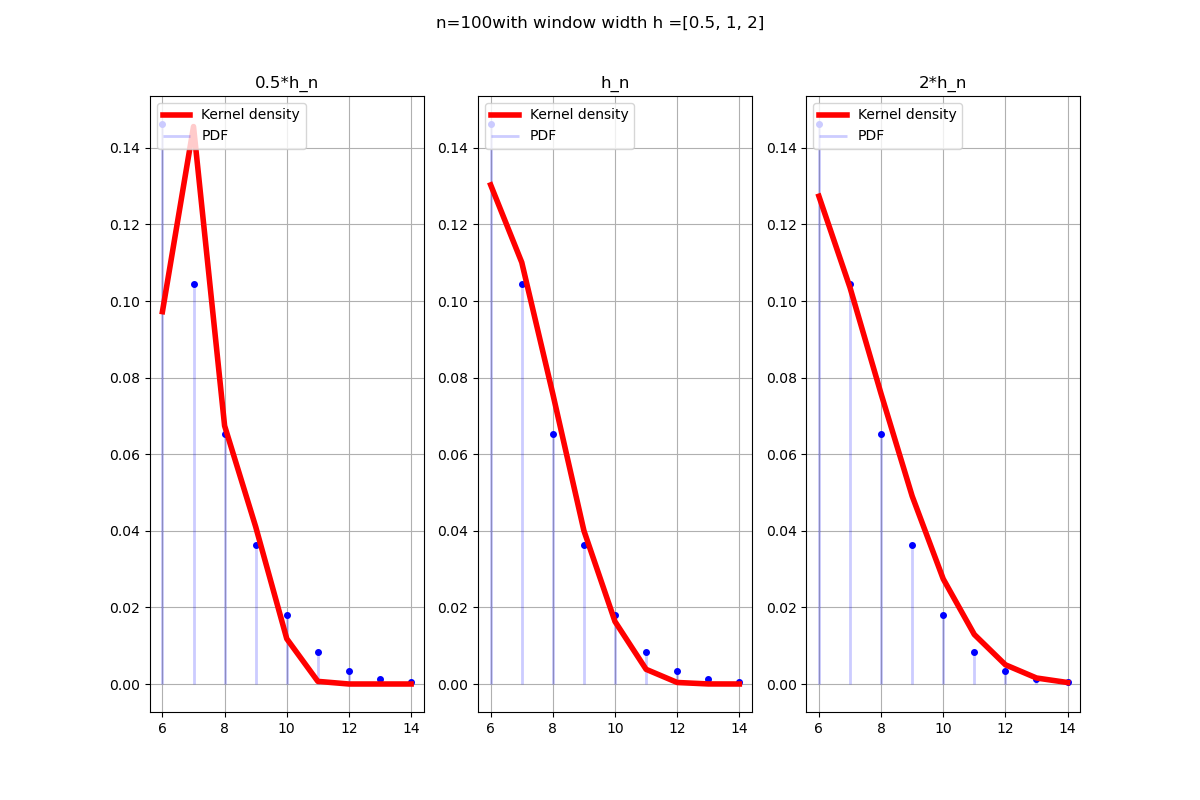
\includegraphics[width=\textwidth]{poisson_pdf_100.png} 
\end{figure}

\begin{figure}[H]
\caption{ Ядерная функция плотности для равномерного распределения n = $20$}
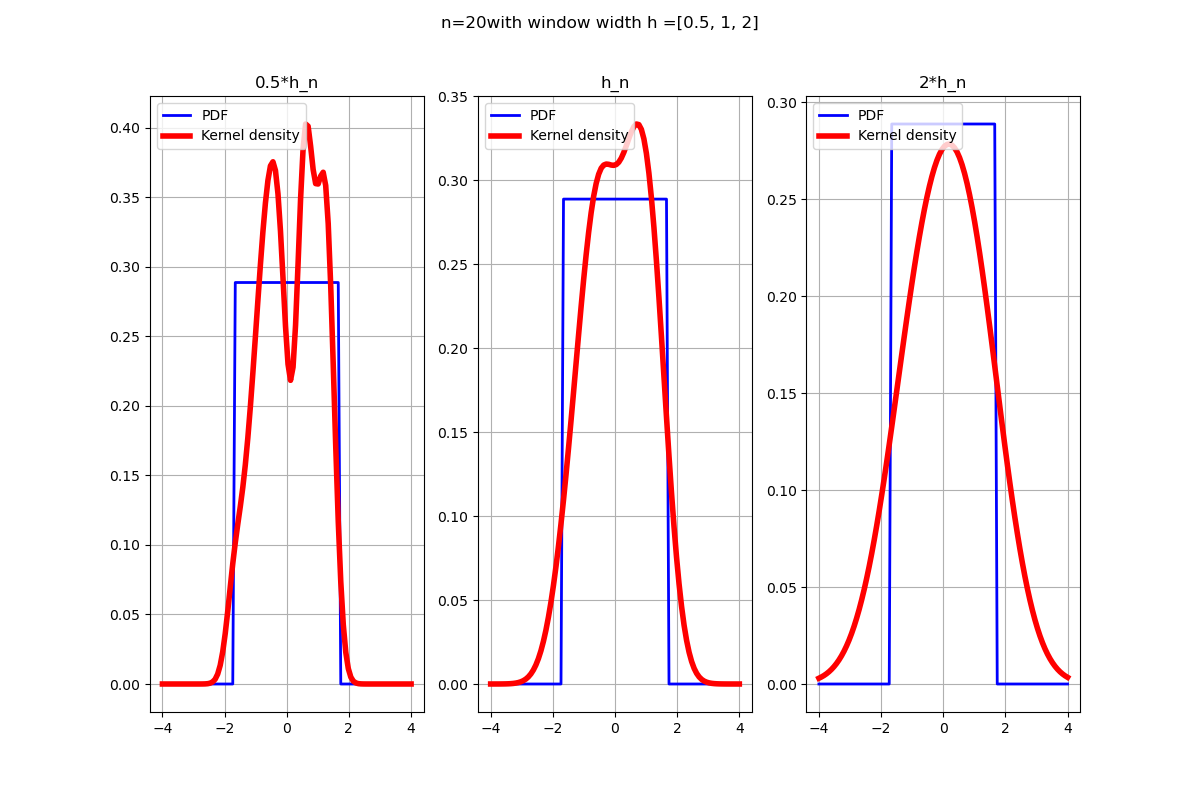
\includegraphics[width=\textwidth]{uniform_pdf_20.png} 
\end{figure}

\begin{figure}[H]
	\caption{ Ядерная функция плотности для равномерного распределения n = $60$}
	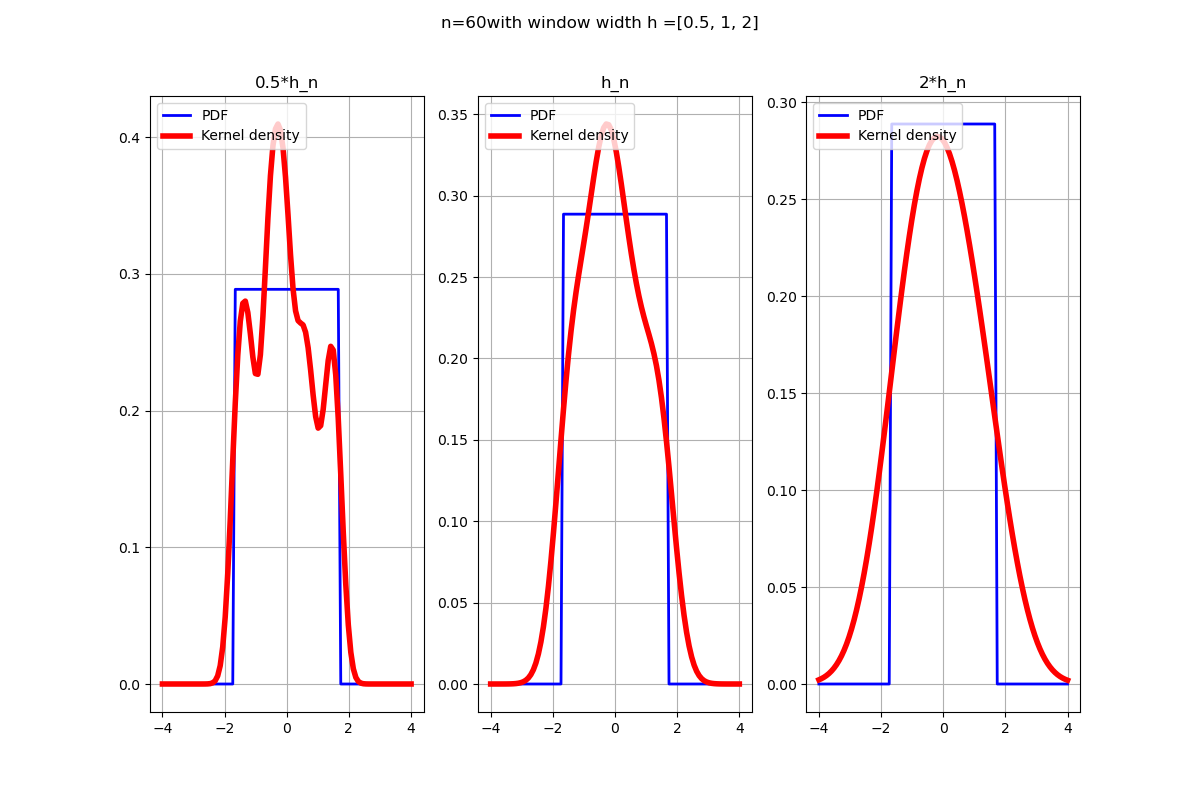
\includegraphics[width=\textwidth]{uniform_pdf_60.png} 
\end{figure}

\begin{figure}[H]
	\caption{ Ядерная функция плотности для равномерного распределения n = $100$}
	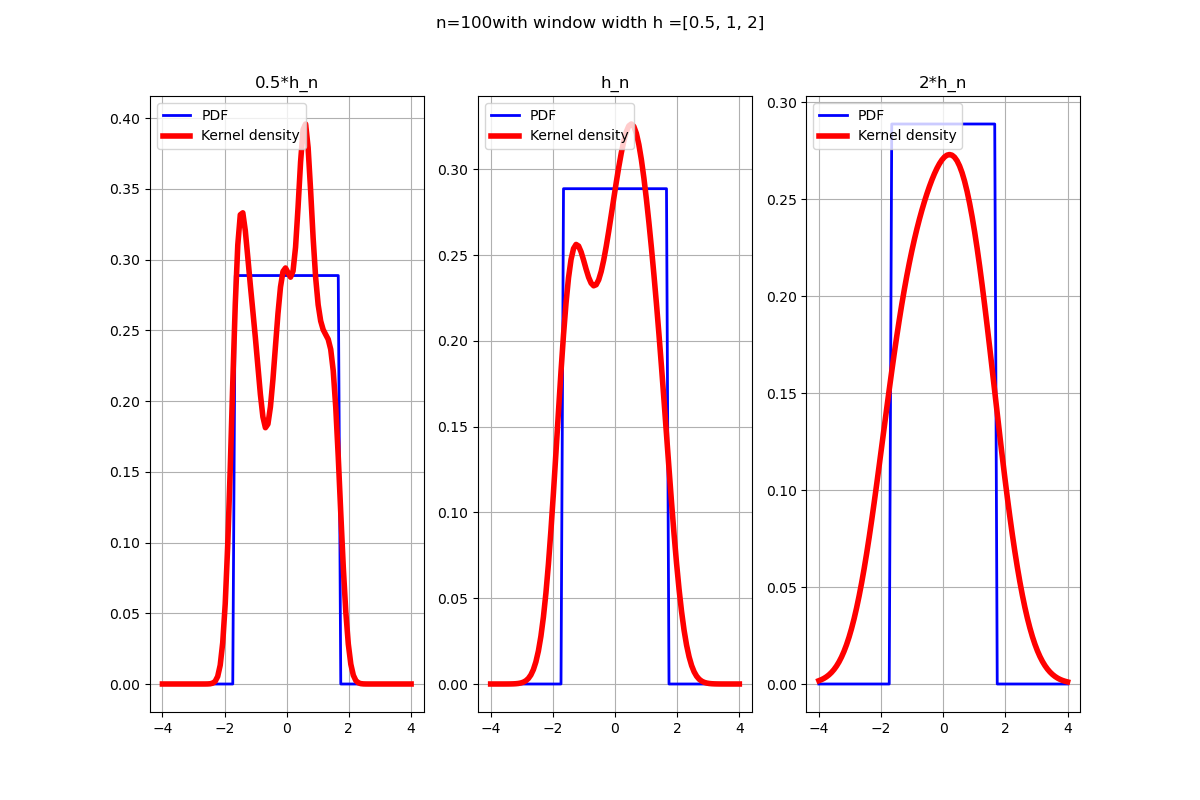
\includegraphics[width=\textwidth]{uniform_pdf_100.png} 
\end{figure}

\end{center}
\subsection{Ядерные функции}
\begin{center}
\begin{figure}[H]
	\caption{Эмпирическая функция для стандартного нормального распределения}
	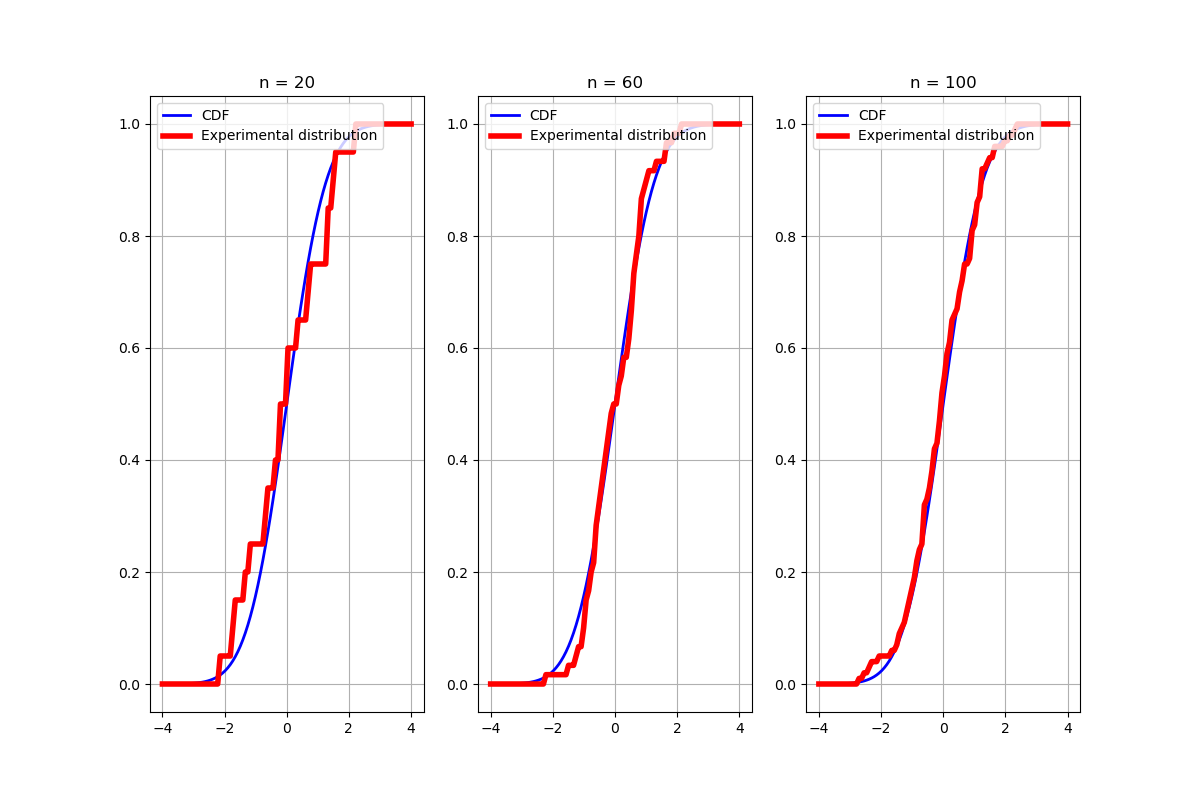
\includegraphics[width=\textwidth]{normal_cdf.png}
\end{figure}
\begin{figure}[H]
	\caption{Эмпирическая функция для стандартного распределения Лапласа}
	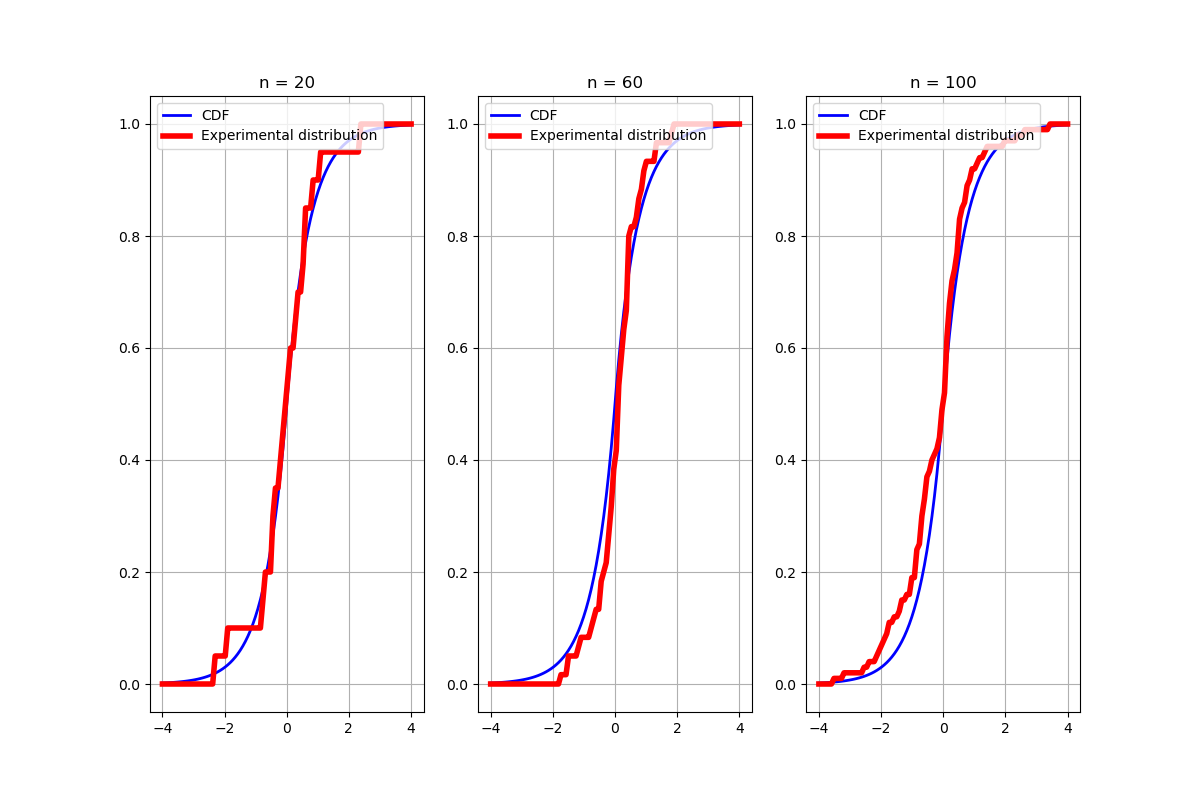
\includegraphics[width=\textwidth]{laplace_cdf.png}
\end{figure}
\begin{figure}[H]
	\caption{Эмпирическая функция для стандартного распределения Коши}
	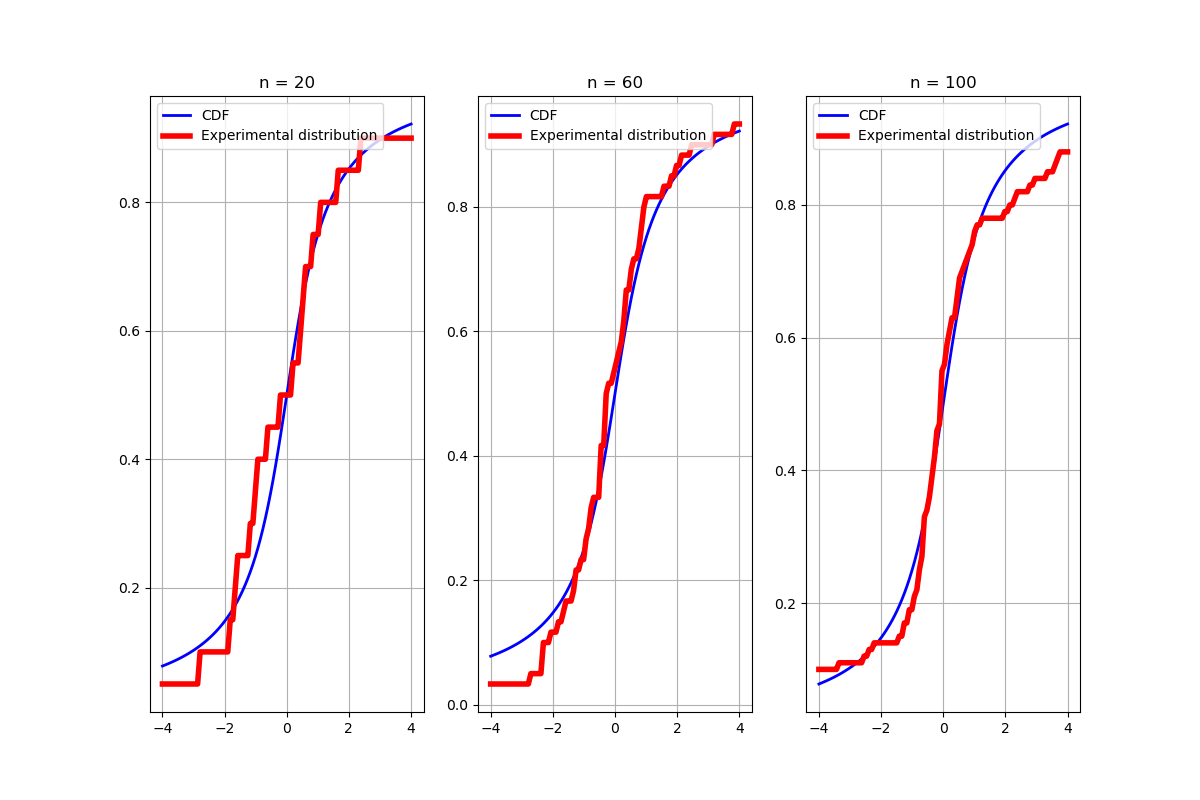
\includegraphics[width=\textwidth]{cauchy_cdf.png}
\end{figure}
 \begin{figure}[H]
	\caption{Эмпирическая функция для распределения Пуассона}
	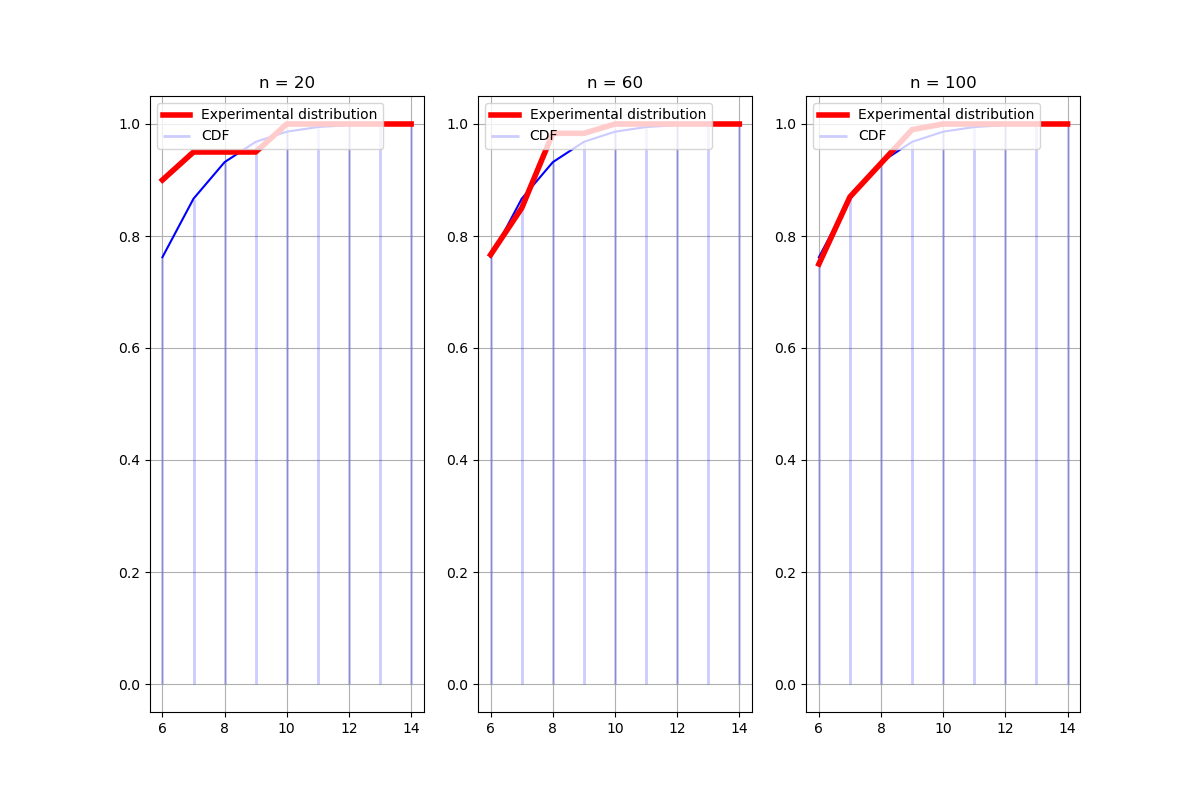
\includegraphics[width=\textwidth]{poisson_cdf.png}
\end{figure}
 \begin{figure}[H]
	\caption{Эмпирическая функция для равномерного распределения}
	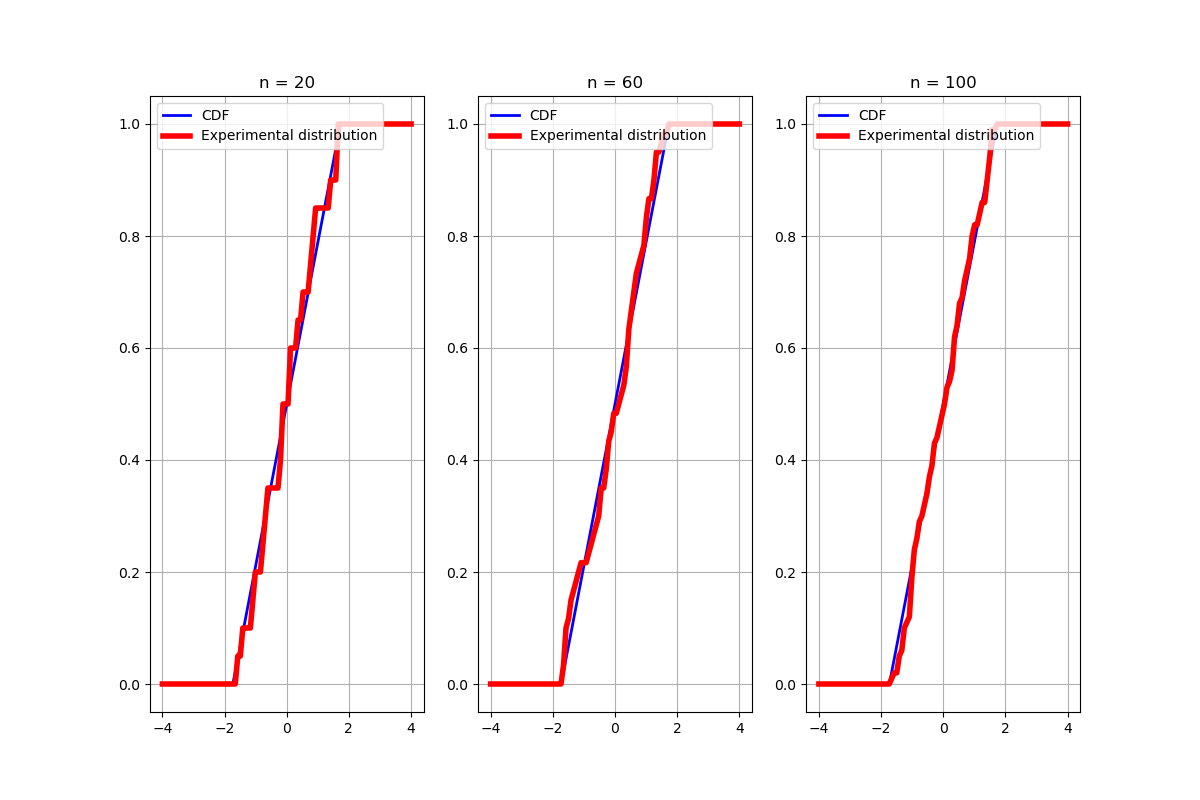
\includegraphics[width=\textwidth]{uniform_cdf.png}
\end{figure}
\end{center}

\section{Выводы}
\par Эмпирическая функция лучше приближает эталонную функцию с ростом объёма выборки.

\par Ядерная оценка функции плотности вероятности с выбранным нормальным ядром лучше всего приближает распределения, близкие к нормальному, с ростом размера выборки качество оценки растёт. Исключением является распределение Коши, так как на относительно больших выборках крайне велики выбросы, которые сильно ухудшают приближение по вариационному ряду. Для улучшения качества приближения можно уменьшить ширину полосы.

\begin{thebibliography}{}    
    \href{https://docs.scipy.org/doc/scipy/reference/stats.html}{Модуль scipy.stats}\\
\end{thebibliography}

\section{Приложения}


Код лаборатрной:\; \url{https://github.com/dkamianskii/MatStatLabs/tree/master/Lab4}


\end{document}